\chapter{Classroom Study}  \label{Chapter:EvaluationInClassroom}
 
This chapter reports on an empirical study of software project telemetry in a classroom setting. The study was conducted in the two software engineering classes taught by Dr. Philip Johnson at the University of Hawaii in Spring 2005: one class for senior-level undergraduate students, and the other for introductory-level graduate students. By curriculum design, the students were divided into groups working on group projects, and introduced software project telemetry as a technique for collecting metrics and performing analyses on their own data. There were 25 study participants. At the end of the study, I distributed a questionnaire to collect the students' opinion about software project telemetry. I also analyzed their telemetry system usage pattern to cross-validate the extent to which their opinions were based on the actual system usage.
	
This chapter begins with a description of the classroom setting in Section \ref{EvaluationInClassroom:Setting}.
Section \ref{EvaluationInClassroom:Role} describes my role in the study.
Section \ref{EvaluationInClassroom:StudyDesign} elaborates on the study design.
Section \ref{EvaluationInClassroom:DataCollection} describes data collection and analysis procedures.
Section \ref{EvaluationInClassroom:Results} reports the results. 
Section \ref{EvaluationInClassroom:Conclusion} concludes the chapter with a summary of the insights learned from this study.







%%%%%%%%%%%%%%%%%%%%%%%%%%%%%%%%%%%%%%%%%%%%%%%%%%%%%%%%%
%                                                       %
%                   S E C T I O N                       %
%                                                       %
%%%%%%%%%%%%%%%%%%%%%%%%%%%%%%%%%%%%%%%%%%%%%%%%%%%%%%%%%

\section{Classroom Setting} \label{EvaluationInClassroom:Setting}

The study was conducted in two software engineering classes: one at the senior undergraduate level (ICS 414), and the other at the introductory graduate level (ICS 613). The two classes followed the same basic curriculum, except that the students at the graduate level were expected to read more supplementary materials and do a more thorough job with their programming assignments. The curriculum had two equally important components:

\begin{itemize}
	\item \textbf{Software Lifecycle Techniques} --- 
The curriculum covered software application lifecycle techniques. They included requirement management, design patterns, change and configuration management, code review and testing. The students were divided into teams of two to four members working on different projects, using tools such as Eclipse (a Java IDE), Ant (a Java build tool), CVS (a configuration management system), and JUnit (a Java unit test framework). The focus was on agile development practice.

	\item \textbf{Software Process Improvement} --- The students were required to collect and analyze their software process and product metrics while performing development tasks. The purpose was to help them acquire hands-on experience in collecting, analyzing, and interpreting software metrics in order to improve their software development processes.
\end{itemize}

The students' software product and process metrics were collected and analyzed using the implementation of software project telemetry introduced in Chapter \ref{Chapter:Implementation}. This was the second semester that the system was used in software engineering classes. A pilot study took place in Fall 2004. 

The software project telemetry system was deployed on a university server where all students created an account to access their metrics data so that they could run telemetry analyses to gain insights into their software development processes. In order to gather product and process metrics, the students were required to instrument their development tools with sensors. These sensors collected a wide variety of information such as the time each project member spent editing source code, the size metrics, the occurrence of unit tests, and the resulting test coverage.

The software project telemetry implementation provides three analysis interfaces: \textit{telemetry chart analysis}, \textit{telemetry report analysis}, and \textit{telemetry expert analysis} (See Section \ref{Implementation:Telemetry:FunctionalDescription}). The telemetry chart and report analyses use predefined telemetry definitions, while the telemetry expert analysis requires the user to use the telemetry language to interact with the system directly. The instructor and I felt that introducing the telemetry language would impose an unnecessary burden on the students. Therefore, we predefined a set of charts and reports that we thought were most useful to them, and only the telemetry chart and report analyses were introduced in class.





%%%%%%%%%%%%%%%%%%%%%%%%%%%%%%%%%%%%%%%%%%%%%%%%%%%%%%%%%
%                                                       %
%                   S E C T I O N                       %
%                                                       %
%%%%%%%%%%%%%%%%%%%%%%%%%%%%%%%%%%%%%%%%%%%%%%%%%%%%%%%%%

\section{Researcher's Role} \label{EvaluationInClassroom:Role}

The instructor of the two software engineering classes in which this study was conducted was Dr. Philip Johnson. He is my dissertation adviser. The software project telemetry system is implemented by me. It was used as a tool by the students to collect and analyze their software product and process metrics. I helped the instructor predefine the telemetry charts and reports that we thought were most useful to the students. However, I did not participate in the teaching of the classes.






%%%%%%%%%%%%%%%%%%%%%%%%%%%%%%%%%%%%%%%%%%%%%%%%%%%%%%%%%
%                                                       %
%                   S E C T I O N                       %
%                                                       %
%%%%%%%%%%%%%%%%%%%%%%%%%%%%%%%%%%%%%%%%%%%%%%%%%%%%%%%%%
\section{Study Design} \label{EvaluationInClassroom:StudyDesign}

The software engineering class was an environment where the use of software project telemetry was mandatory by curriculum design. An important goal of the class was to let the students gain experience with metrics-driven process improvement. This provided a good opportunity for me to gather opinions about software project telemetry from a relatively large number of users with relatively diverse backgrounds.

The study was a mixed-methods study. The goal was to explore the way the students used software project telemetry and the problems they encountered during their use in a natural setting. There were 25 students enrolled in the two classes. Following them around and observing how they interacted with the technology to make process improvement decisions was not a feasible choice. Therefore, I decided to use a survey to collect their opinions. The interview method was not chosen to conduct the survey because of the concern that the students might feel pressured to give more favorable opinions due to the involvement of the professor in the research, and thus bias the study results. Instead, a questionnaire was used. It has the advantage of ease of administration and rapid turn around in data collection. The disadvantage is that the questions I can ask are fixed and limited in a questionnaire.

The questionnaire was administered less than one week before the final examination. To further mitigate the threat that the students might be concerned that their responses would influence their grades and thus comment more favorably toward software project telemetry, I made the questionnaire anonymous, instructed the students specifically not to reveal their names in their responses, and assured them that their responses would only be processed after their instructor had turned in their final grades.
	
The decision to use a questionnaire, at the same time, implied that I had to rely on the students' self-reported opinions to evaluate software project telemetry. The threat was mitigated through cross-validation. The usage of the software project telemetry system was logged. If the survey responses were mostly positive and the log indicated that the students ran the analyses frequently or regularly, or if the survey responses were mostly negative and the log indicated that the students stopped using the system after a while, I could put more confidence in the responses because their opinions were consistent with the actual system usage pattern. On the other hand, if it turned out that the students opinions were very positive but they all stopped using the system after a while, then I had to question their responses because the actual system usage pattern was inconsistent with their opinions. My cross-validation was partial in nature, because I could not match the students' telemetry analysis invocation data to individual responses due to the chosen design of anonymous questionnaire.






%%%%%%%%%%%%%%%%%%%%%%%%%%%%%%%%%%%%%%%%%%%%%%%%%%%%%%%%%
%                                                       %
%                   S E C T I O N                       %
%                                                       %
%%%%%%%%%%%%%%%%%%%%%%%%%%%%%%%%%%%%%%%%%%%%%%%%%%%%%%%%%

\section{Data Collection and Analysis} \label{EvaluationInClassroom:DataCollection}

This study collected data from two sources:
\begin{itemize}
	\item A survey questionnaire was distributed on the last day of instruction asking the students their opinions about software project telemetry.
	\item The software project telemetry system was instrumented. All usage information was logged.
\end{itemize}

The two sources of data were integrated at data interpretation phase, and priority was given to the analysis of the questionnaire responses. The software project telemetry system log was used to assess the extent to which the students' opinions were based on the actual system usage.




\subsection{Survey Questionnaire} \label{EvaluationInClassroom:Survey}

The survey was conducted through an anonymous written questionnaire administered on the last day of instruction. The questions covered metrics collection overhead, analysis usability and utility, and the students' perception of whether software project telemetry was a reasonable approach to process improvement and project management in ``real world'' settings.

Each question was represented by a statement. For example, when collecting information about telemetry analysis utility, I made the statement \textit{``telemetry analyses have shown me valuable insight into my and my team's software development process''}. Then, I asked the students to rank their feelings toward the statement:

\begin{itemize}
  \setlength{\itemsep}{0pt}
  \setlength{\parskip}{0pt}
	\item Strongly Disagree
	\item Disagree
	\item Neutral
	\item Agree
	\item Strongly Agree
	\item Not Applicable
\end{itemize}

The last option \textit{``not applicable''} was provided to allow the students to skip the questions which they were unable to answer or they did not want to answer. At the end of each question, I provided large empty space for them to write down any related comments such as justification or elaboration of the answer. The last part of the questionnaire was a free response section where the students were encouraged to provide any additional suggestions or comments. The actual questionnaire is attached in Appendix \ref{Appendix:EvaluationInClassroom} for reference.

%such as their general opinions toward software measurement, their concerns about the way software project telemetry handled their personal process data, their suggestions on how the system could be improved, etc.

\subsection{System Usage Log} \label{EvaluationInClassroom:InvocationLog}

The software project telemetry system exposes a web interface though which the users could invoke telemetry analyses over their software product and process metrics. The system deployed for classroom use was instrumented with an automatic logging facility. Telemetry analysis invocation information, such as time, user name, and full web request parameters, were logged.









%%%%%%%%%%%%%%%%%%%%%%%%%%%%%%%%%%%%%%%%%%%%%%%%%%%%%%%%%
%                                                       %
%                   S E C T I O N                       %
%                                                       %
%%%%%%%%%%%%%%%%%%%%%%%%%%%%%%%%%%%%%%%%%%%%%%%%%%%%%%%%%
\clearpage
\section{Results} \label{EvaluationInClassroom:Results}

All of the 25 students enrolled in the two software engineering classes participated in the questionnaire, of which 9 were from the senior undergraduate level class and 16 were from the introductory graduate level class. The students had a fairly diverse background. Their total programming experience, as defined from their first \textit{``Hello World''} application, ranged from 3 to 25 years, with a mean of 6.92 and a standard deviation of 4.43. Their paid professional experience\footnote{I specifically asked the students to exclude the experience from half-time or less than half-time on-campus employment, such as student helper or research assistant, even if they were paid to program.} ranged from 0 to 8 years, with a mean of 1.27 and a standard deviation of 2.10.\footnote{One student did not answer this single question and thus was not included in the statistics regarding professional background.} The survey was conducted in a normal class session on the last day of instruction, and the response rate was 100\%.


\subsection{Results from Individual Survey Question}

The survey questions are listed below along with the results. Each question was in the form of a statement, and the students were asked to choose the answer that most closely matched their feelings about the statement. Their choices were: \textit{strongly disagree}, \textit{disagree}, \textit{neutral}, \textit{agree}, \textit{strongly agree}, and \textit{not applicable}. The resulting statistics were computed by excluding the \textit{``not applicable''} answers.


\setlength{\parindent}{0mm} %indentation of paragraphs

\clearpage
\subsubsection{Statement 1: I have no trouble installing and configuring the sensors.}

\textbf{\textit{Elaboration of the Statement:}} 
Software project telemetry uses sensors to collect metrics. The sensors must be installed and properly configured by the developers. The question was designed to gather information about the one-time installation and setup cost of the sensors. 

\begin{quote}\end{quote} % make some lines

\begin{figure}[h]
  \center
  \includegraphics[width=0.50\textwidth]{figures/ClassroomSurvey-Q1}
  \label{fig:InClassSurvey-Q1}
\end{figure}

\begin{center}\textbf{Response Rate:} 25 out of 25\end{center}
\begin{table}[h]
	\centering
		\begin{tabular}{|c|c|c|c|c|} 
			\hline
			\textbf{Strongly Disagree} & \textbf{Disagree} & \textbf{Neutral} & \textbf{Agree} & \textbf{Strongly Agree} \\
			\hline
			\textit{1} & \textit{10} & \textit{3} & \textit{6} &\textit{5} \\
			\hline
		\end{tabular}
	\label{table:InClassSurvey-Q1}
\end{table}

\textbf{\textit{Explanation of the Result:}}
It turned out that sensor installation and configuration involved quite complex procedures. 40\% of the respondents did not agree with the statement. One of the students even responded: \textit{``I still have problems with some sensors (at the end of the semester).''} Most students expressed the wish to have an all-in-one intelligent graphical user interface to install and configure the sensors.

%3.16 (1.28) [1, 5]
%*I didn't read much documentation. I followed directions in class.
%*I thought the instructions were much too detailed. I got lost with details.
%*No all-in-one installer. To much manual work.
%*It took some time to install it.
%*Should really consider creating installer scripts.
%*I could not figure out that I need to put sensor.properties to .hackystat folder.
%*I still have problems with some sensors.
%*Problem with regional time format settings.
%*Not hard, just sometimes it seemed data didn't show up.
%*Need GUI driver process. 


\clearpage
\subsubsection{Statement 2: After sensors are installed and configured, there is no overhead collecting metrics.}

\textbf{\textit{Elaboration of the Statement:}}
Once installed, sensors collect metrics automatically. This question was designed to gather information about the long term chronic metrics collection overhead (excluding the one-time setup cost).

\begin{quote}\end{quote} % make some lines

\begin{figure}[h]
  \center
  \includegraphics[width=0.50\textwidth]{figures/ClassroomSurvey-Q2}
  \label{fig:InClassSurvey-Q2}
\end{figure}

\begin{center}\textbf{Response Rate:} 24 out of 25\end{center}
\begin{table}[h]
	\centering
		\begin{tabular}{|c|c|c|c|c|} 
			\hline
			\textbf{Strongly Disagree} & \textbf{Disagree} & \textbf{Neutral} & \textbf{Agree} & \textbf{Strongly Agree} \\
			\hline
			\textit{0} & \textit{0} & \textit{6} & \textit{7} &\textit{11} \\
			\hline
		\end{tabular}
	\label{table:InClassSurvey-Q2}
\end{table}

\textbf{\textit{Explanation of the Result:}}
The sensor-based metrics collection approach adopted in software project telemetry appeared to have achieved its design goal of eliminating long-term chronic data collection overhead. No one disagreed with the statement.


%4.21 (0.83) [3, 5] (one answered N/A)
%*Problems occurred with the new sensors themselves. They failed to collect/send data.
%*Sometimes the sensor do not send data and you don't know until late.
%*Broadband won't feel a thing.


\clearpage
\subsubsection{Statement 3: It's simple to invoke predefined telemetry chart and report analyses.}

\textbf{\textit{Elaboration of the Statement:}}
The telemetry chart and report analysis used in the class did not require the students to use the telemetry language. Instead, the instructor and I predefined a set of useful telemetry charts and reports for them. This question was designed to gather information about the usability of the two telemetry analysis interfaces.

\begin{quote}\end{quote} % make some lines

\begin{figure}[h]
  \center
  \includegraphics[width=0.50\textwidth]{figures/ClassroomSurvey-Q3}
  \label{fig:InClassSurvey-Q3}
\end{figure}

\begin{center}\textbf{Response Rate:} 24 our of 25\end{center}
\begin{table}[h]
	\centering
		\begin{tabular}{|c|c|c|c|c|} 
			\hline
			\textbf{Strongly Disagree} & \textbf{Disagree} & \textbf{Neutral} & \textbf{Agree} & \textbf{Strongly Agree} \\
			\hline
			\textit{0} & \textit{2} & \textit{5} & \textit{11} &\textit{6} \\
			\hline
		\end{tabular}
	\label{table:InClassSurvey-Q3}
\end{table}

\textbf{\textit{Explanation of the Result:}}
Though most students appreciated the idea of being able to run metrics analysis by choosing from a list of predefined telemetry charts and reports, they thought the telemetry analysis interface could be further improved. It turned out that a major problem involved the input of analysis parameter values. Different telemetry charts or reports had different parameter requirements, but it was hard to tell from the simple web interface what parameters were expected.




%3.88 (0.90) [ 2-5] (one answered N/A)
%*Some tasks are somewhat not visible.
%*Some require unknown parameters.
%*Some. Others require parameters, but no instructions on what those parameters might be.
%*They don't work so well due to the last parameter option. What goes there? How about a help link for each option?
%*The report names aren't that descriptive, and the the parameters needed were confusing.

\clearpage
\subsubsection{Statement 4: Telemetry analyses have shown me valuable insight into my and / or my team's software development process.}

\textbf{\textit{Elaboration of the Statement:}}
One of the goals of software project telemetry is to make development process transparent so that problem can be detected early. This question was designed to measure whether software project telemetry had achieved that goal or not.

\begin{quote}\end{quote} % make some lines

\begin{figure}[h]
  \center
  \includegraphics[width=0.50\textwidth]{figures/ClassroomSurvey-Q4}
  \label{fig:InClassSurvey-Q4}
\end{figure}

\begin{center}\textbf{Response Rate:} 25 out of 25\end{center}
\begin{table}[h]
	\centering
		\begin{tabular}{|c|c|c|c|c|} 
			\hline
			\textbf{Strongly Disagree} & \textbf{Disagree} & \textbf{Neutral} & \textbf{Agree} & \textbf{Strongly Agree} \\
			\hline
			\textit{0} & \textit{0} & \textit{5} & \textit{10} &\textit{10} \\
			\hline
		\end{tabular}
	\label{table:InClassSurvey-Q4}
\end{table}

\textbf{\textit{Explanation of the Result:}}
No one disagreed with the statement. The numbers appeared to indicate that software project telemetry had achieved the goal of making development process transparent. In fact, some of the students appeared to suggest that it made their process more transparent than they had wished by expressing concerns about their data privacy.


%4.20 (0.76) [3-5]
%*Mostly it shows who doesn't work.
%*Dr. Johnson can track our progress. Yikes!.
%*Have not done enough projects to get a pattern.
%*Sometimes the data is not precise.
%*Makes me more aware of what others are doing (good or bad)
%*Good tool.


\clearpage
\subsubsection{Statement 5: Telemetry analyses have helped me improve my software development process.}

\textbf{\textit{Elaboration of the Statement:}}
This question was designed to ask the students whether there was any self-perceived process improvement as a result of using software project telemetry. In other words, it tried to determine the causal relationship between software project telemetry and process improvement.

%Software project telemetry helps a developer improve his/her development process by making the development process transparent and the information available to the user, but it cannot make process improvement decisions on behalf of the user. Whether a developer can improve his/her development process depends crucially on (1) his/her ability to interpret telemetry results and take actions accordingly, and (2) whether telemetry analysis is able to deliver the relevant information in an easy-to-understand way. 

\begin{quote}\end{quote} % make some lines

\begin{figure}[h]
  \center
  \includegraphics[width=0.50\textwidth]{figures/ClassroomSurvey-Q5}
  \label{fig:InClassSurvey-Q5}
\end{figure}

\begin{center}\textbf{Response Rate:} 25 out of 25\end{center}
\begin{table}[h]
	\centering
		\begin{tabular}{|c|c|c|c|c|} 
			\hline
			\textbf{Strongly Disagree} & \textbf{Disagree} & \textbf{Neutral} & \textbf{Agree} & \textbf{Strongly Agree} \\
			\hline
			\textit{1} & \textit{2} & \textit{6} & \textit{13} &\textit{3} \\
			\hline
		\end{tabular}
	\label{table:InClassSurvey-Q5}
\end{table}

\textbf{\textit{Explanation of the Result:}}
Most students thought that telemetry analyses had helped them improve their software development process. However, due to the limitation of this study, there is no conclusive evidence to determine whether the students' self-perceived process improvement was due to the use of telemetry analyses on their metrics, or the fact that they learned new development best practice in class, or both.

%3.6 (0.96) [1-5]
%The first key is that analyses have made me aware.
%During the development, not really. Afterwards, it's fun to look at it.
%Maybe consider more information gathering to give programmers insights v.s. giving manager insight.
%(Telemetry analyses have helped me improve my software development process) compared to what I learned in class, from students, and on the web.


\clearpage
\subsubsection{Statement 6: If I was a professional software developer, I will want to use telemetry analyses in my development projects.}

\textbf{\textit{Elaboration of the Statement:}}
This question was designed to ask the students whether they perceived software project telemetry as a reasonable approach to process improvement in ``real'' development settings from the perspective of \textit{a developer}. 

\begin{quote}\end{quote} % make some lines

\begin{figure}[h]
  \center
  \includegraphics[width=0.50\textwidth]{figures/ClassroomSurvey-Q6}
  \label{fig:InClassSurvey-Q6}
\end{figure}

\begin{center}\textbf{Response Rate:} 25 out of 25\end{center}
\begin{table}[h]
	\centering
		\begin{tabular}{|c|c|c|c|c|} 
			\hline
			\textbf{Strongly Disagree} & \textbf{Disagree} & \textbf{Neutral} & \textbf{Agree} & \textbf{Strongly Agree} \\
			\hline
			\textit{1} & \textit{1} & \textit{7} & \textit{11} &\textit{5} \\
			\hline
		\end{tabular}
	\label{table:InClassSurvey-Q6}
\end{table}

\textbf{\textit{Explanation of the Result:}}
The majority of the students confirmed the value of software project telemetry as an approach to metrics-based process improvement. However, some of them expressed the concern about sharing private personal process data with others. For example, one student said: \textit{``I don't want to show the data to my boss.''}


%3.72 (0.98) [1-5]
%*Only after getting more experience with the tool would I feel confortable to use it in a prefessional development environment.
%*I'll be concetrating on my work. Stats don't really matter.
%*I don't want to show the data to my boss.
%*More useful for management.
%*Only if I was in a development team. If I was alone I am not sure I'd use it.


\clearpage
\subsubsection{Statement 7: If I was a project manager, I will want to use telemetry analyses in my development projects.}

\textbf{\textit{Elaboration of the Statement:}}
This question was designed to ask the students whether they perceived software project telemetry as a reasonable approach to project management and process improvement in ``real'' development settings from the perspective of \textit{a project manager}. 

\begin{quote}\end{quote} % make some lines

\begin{figure}[h]
  \center
  \includegraphics[width=0.50\textwidth]{figures/ClassroomSurvey-Q7}
  \label{fig:InClassSurvey-Q7}
\end{figure}

\begin{center}\textbf{Response Rate:} 25 out of 25\end{center}
\begin{table}[h]
	\centering
		\begin{tabular}{|c|c|c|c|c|} 
			\hline
			\textbf{Strongly Disagree} & \textbf{Disagree} & \textbf{Neutral} & \textbf{Agree} & \textbf{Strongly Agree} \\
			\hline
			\textit{0} & \textit{0} & \textit{3} & \textit{12} &\textit{10} \\
			\hline
		\end{tabular}
	\label{table:InClassSurvey-Q7}
\end{table}

\textbf{\textit{Explanation of the Result:}}
The data appeared to overwhelmingly suggest that software project telemetry was a valuable tool for project managers. The result seemed to be consistent with the finding in Statement 4 that software project telemetry achieved the goal of making development process transparent. It also seemed to confirm the recurring theme in the answers to Statement 6 that developers worried about their privacy. 



%4.28 (0.68) [3-5]
%*See above comment - would add training of development team. (above comment refers to the student's comment for Q6: Only after getting more experience with the tool would I feel confortable to use it in a prefessional development environment).
%*I want to know what people are doing.
%*Can gather data for future projects.



\setlength{\parindent}{6mm} %indentation of paragraphs


\clearpage
\subsection{Results from Free Response Section}

The students provided a lot of textual feedback. I identified several themes: some were positive, some were negative. They are all listed below in bold face followed by the actual comments from the students.

\subsubsection{\textit{Metrics Collection:}}
\begin{itemize}
	\item \textbf{Sensor-based automated and unobtrusive metrics collection is effortless.}
    \begin{quote} \textit{``Overall it is an incredible tool that generally makes 
           software development metric collection effortless.''}\end{quote}
 
  \item \textbf{Sensor installation and configuration are too complex.}
    \begin{quote} \textit{``It took some time to install it.''} \end{quote}
    \begin{quote} \textit{``I thought the instructions were much too 
           detailed. I got lost with details.''} \end{quote}
    \begin{quote} \textit{``No all-in-one installer. Too much manual 
           work.''} \end{quote}  
    \begin{quote} \textit{``I could not figure out that I need to put 
           sensor.properties to .hackystat folder.''} \end{quote}
    \begin{quote} \textit{``I still have problems with some sensors
           (at the end of the semester).''} \end{quote} 
    \begin{quote} \textit{``Please make the installation process 
           easier.''} \end{quote}
    \begin{quote} \textit{``(It) should have some mechanism to switch on 
           the sensors easily instead of going into the sensor property file 
           to change the true to false.''} \end{quote}
    \begin{quote} \textit{``(You) should really consider creating 
           installer scripts.''} \end{quote}  
    \begin{quote} \textit{``(They) need GUI driver process.''} \end{quote}           
           

  \item \textbf{Some sensors do not seem to work correctly.}  
    
    Comment: This is a complex issue. Several reasons have been identified that could cause sensors seemingly not working as expected:
    (1) programming bugs in sensor code, 
    (2) incorrect sensor configurations or project settings, 
    or (3) inappropriate interpretation of metrics data.
  
    \begin{quote} \textit{``The sensors of the Jupiter does not work 
           correctly sometimes, and did not sense any data and send 
           it to the server.''} \end{quote}
    \begin{quote} \textit{``I had a lot of problems getting Jblanket 
           to work on a web page with http unit. For some version, 
           it kept closing the web application from running on the server, 
           even with no dependencies.''} \end{quote}  
    \begin{quote} \textit{``I spend 2 hours one night to debug a problem 
           with the Ant build file and end up with only 15 minutes
           on Hackystat.''} \end{quote}

\end{itemize}






\subsubsection{\textit{Metrics Analysis:}}
\begin{itemize}
  \item \textbf{Software project telemetry makes development process transparent.}
    \begin{quote} \textit{``There is powerful information and insights 
           to gain.''} \end{quote} 
    \begin{quote} \textit{``The first key is that analyses have made 
           me aware.''} \end{quote}
    \begin{quote} \textit{``(Telemetry analyses have helped me improve 
           my software development process) compared to what I learned 
           in class, from students, and on the web.''} \end{quote}
    \begin{quote} \textit{``(Telemetry analysis) makes me more aware of 
           what others are doing -- good or bad?''} \end{quote}
    

  \item \textbf{Telemetry data interpretation is the key to get the value from the tool.}
    \begin{quote} \textit{``I would say that understanding and interpreting 
           the results to benefit the development process is the key ingredient 
           to getting value from the data. Does a team of software developers 
           understand the domain to make use of the information?''} \end{quote}
    \begin{quote} \textit{``Have not done enough projects to get a
           pattern.''} \end{quote}
 
  \item \textbf{Software project telemetry is better suited as a manager's tool than as a developer's tool.} 
    \begin{quote} \textit{``(It is) more useful for management.''} \end{quote}  
    \begin{quote} \textit{``I want to know what people are doing.''} \end{quote}
    
  \item \textbf{The web interface for telemetry analysis can be made more user-friendly.}
    \begin{quote} \textit{``The website interface is really improvable.''} \end{quote}
    \begin{quote} \textit{``I think the Hackystat server website can be more user
           friendly. It took me a while to get used to the page and find the 
           relevant (telemetry) charts I wanted.''} \end{quote}  
    \begin{quote} \textit{``The user interface is a little bit confusing. 
           It's hard to click on Extras (link) when there is no information about 
           what Extra (link) does.''} \end{quote}
    \begin{quote} \textit{``Interface to Hackystat website 
          (for telemetry analysis) yields too many options on pages. 
           Could use a simplified design.''} \end{quote}
    \begin{quote} \textit{``I think the way a developer views a (telemetry) report 
           needs to be simplified. Of course, I can see some people would want to
           customize their own (telemetry) reports.''} \end{quote}  
    \begin{quote} \textit{``Some (telemetry analysis invocation) require 
           unknown parameters.''} \end{quote}
    \begin{quote} \textit{``Others (telemetry analysis invocations) require 
           parameters, but no instructions on what those parameters 
           might be.''} \end{quote}
    \begin{quote} \textit{``They (telemetry analysis invocations) don't work 
           so well due to the last parameter option. What goes there? 
           How about a help link for each option?''} \end{quote}  
    \begin{quote} \textit{``The (telemetry) report names aren't that descriptive, 
           and the parameters needed were confusing.''} \end{quote}   
             
\end{itemize}







\subsubsection{\textit{Privacy Concern:}}
\begin{itemize}
  \item \textbf{Developers have concerns about the privacy of their personal process data.}
    \begin{quote} \textit{``(Software project telemetry data are) good
           if used correctly.''} \end{quote}
    \begin{quote} \textit{``(Telemetry analyses) makes me more aware of 
           what others are doing -- good or bad?''} \end{quote}
    \begin{quote} \textit{``I don't want to show the data to my 
           boss.''} \end{quote}
    \begin{quote} \textit{``Maybe (you should) consider more information 
           gathering to give programmers insights v.s. giving manager 
           insight.''} \end{quote}
\end{itemize}
  
  
   


\subsubsection{\textit{Uncategorized:}}
\begin{itemize} 
  \item \textbf{Uncategorized}   
    \begin{quote} \textit{``Eclipse sensor updates too often. 
           Every time when I start Eclipse I had to download new version. 
           It was too much overhead for me. But I do not want to disable 
           automatic update, because I will forget to update if it is 
           disabled. Can you limit the sensor updates to once a week or 
           twice a month?''} \end{quote}  
    \begin{quote} \textit{``I'll be concentrating on my work. Stats don't 
           really matter.''} \end{quote}     
    \begin{quote} \textit{``(Telemetry analysis is useful) only if I was 
           in a development team. If I was alone I am not sure 
           I'd use it.''} \end{quote} 
\end{itemize}





\subsection{Results from Telemetry Analysis Invocation Log}
\label{EvaluationInClassroom:Results:InvocationLog}

The automatic logging facility in the software project telemetry system recorded all analysis requests in space-delimited files. I wrote a simple application parsing the log files and imported the data into a Microsoft Access database. I then ran SQL query inside Access and exported the results into a Microsoft Excel file. From there, I used pivot table slicing the data. The final results were presented in Figure \ref{fig:ClassroomStudyTotalInvocation} and \ref{fig:ClassroomStudyIndividualInvocation}.

Figure \ref{fig:ClassroomStudyTotalInvocation} showed the total number of telemetry analysis invocations by all the students participating in this study. The number of invocations increased steadily from 47 in January to 967 in April. However, there was a sharp decrease in the number in May, which was 101. The decrease could be explained by the fact that Spring semester ended in that month and final examinations were all scheduled in the second week by the University. 

The numbers clearly showed a pattern of increased utilization of telemetry analysis over time by the students. There were two plausible explanations: (1) telemetry analysis got more interesting when there were more metrics data available, and (2) it took some time for the students to realize the benefit of software project telemetry.

Figure \ref{fig:ClassroomStudyIndividualInvocation} broke the numbers in Figure \ref{fig:ClassroomStudyTotalInvocation} further by individual student. Overall, the individual student's telemetry analysis invocation followed the same pattern as in Figure \ref{fig:ClassroomStudyTotalInvocation}: steady increase in the number from January to April, and a sharp drop in May due to final examinations.  There were 25 study participants, but Figure \ref{fig:ClassroomStudyIndividualInvocation} indicated that one student had never invoked telemetry analysis. Since the survey questionnaire was anonymous, I was unable to match the individual student's analysis invocation information to his/her survey response.

Interestingly, 60\% of the students did not invoke telemetry analysis during the first two months: January and Feburary. However, in March and April, almost everybody invoked telemetry analysis a lot (of course, except the 25th student who had never run a single analysis). The numbers seemed to suggest that software project telemetry was indeed useful to the students once their historical metrics data had reached certain threshold. It was no surprise, since historical metrics data were used to establish a baseline for comparison in software project telemetry.

My final conclusion was that the students' telemetry analysis invocation pattern were consistent with the overall positive tune in their survey responses. It assured my confidence in the subjective opinions from the students about software project telemetry.

\begin{figure}[tbp]
  \centering
  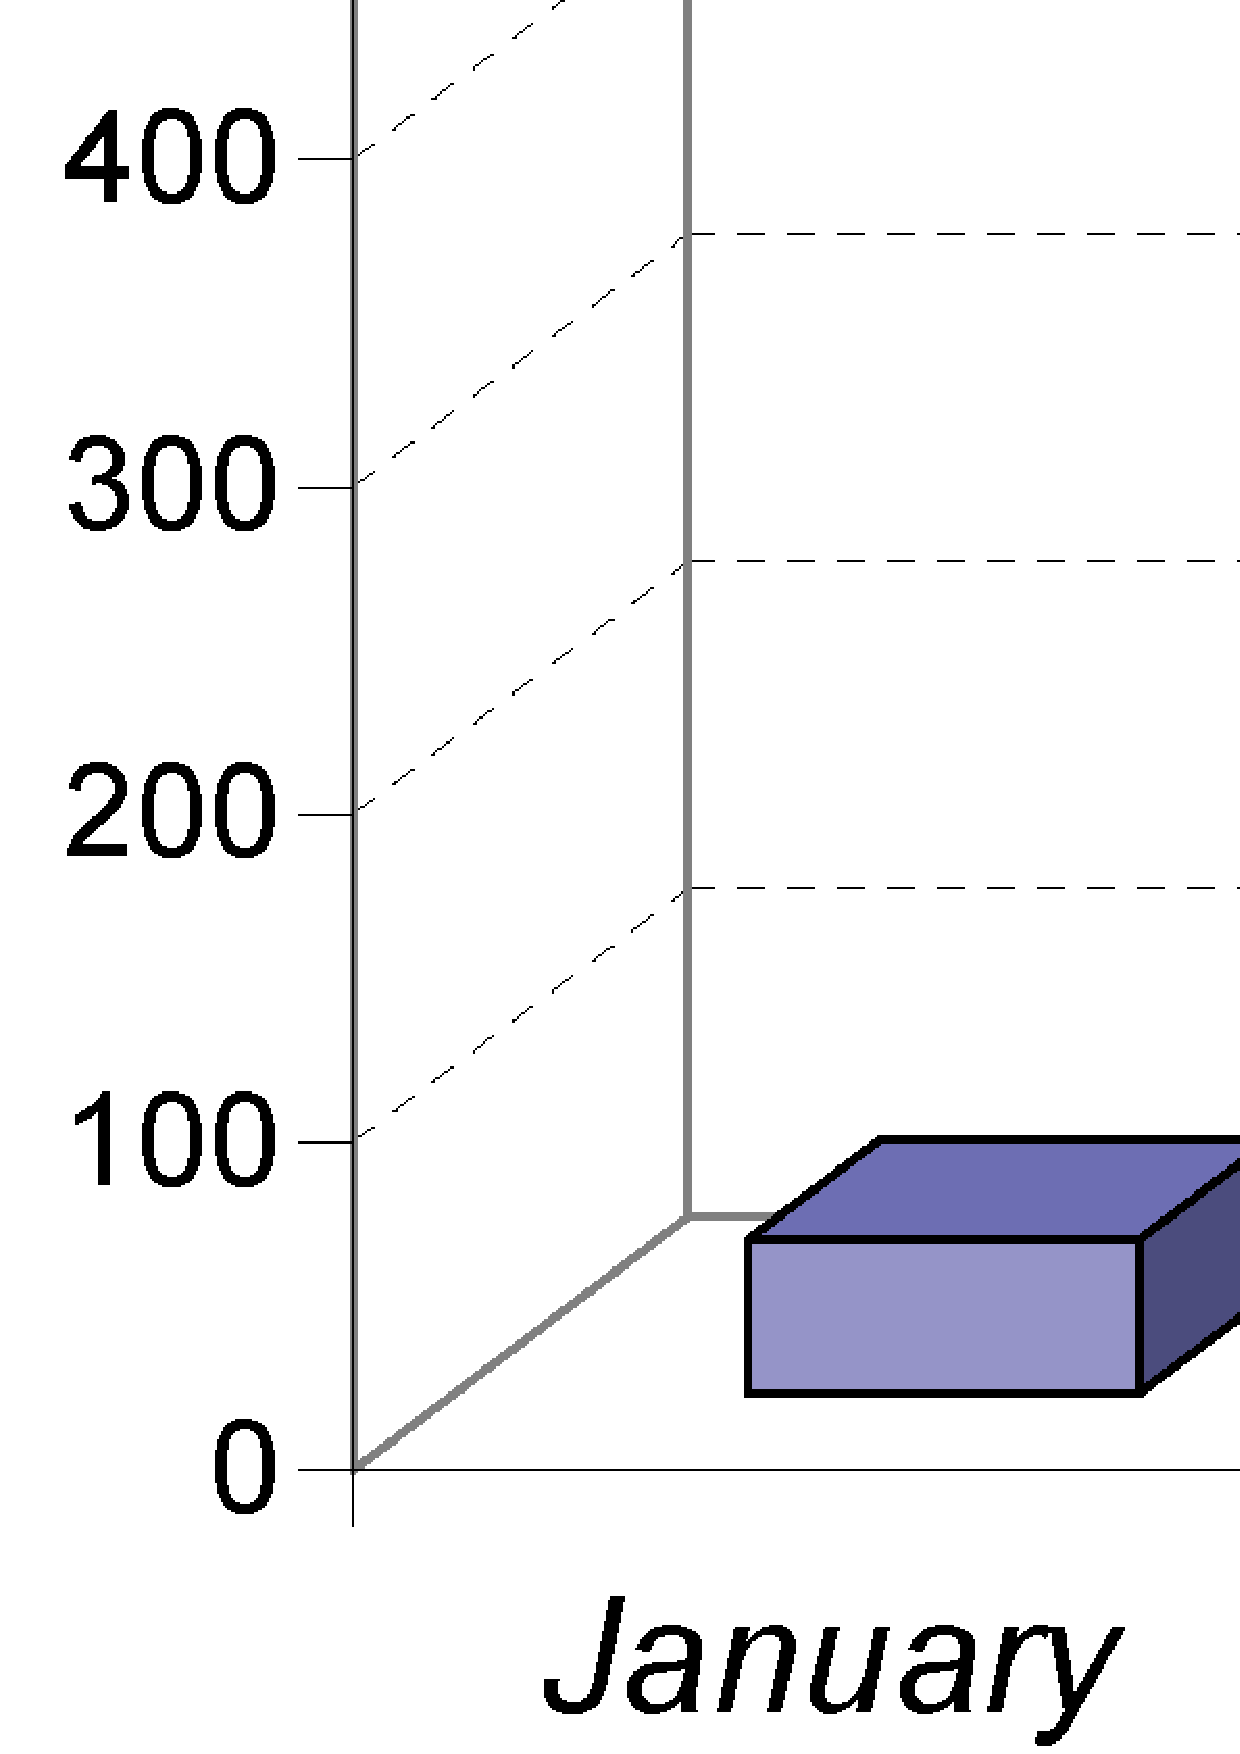
\includegraphics[width=1.00\textwidth]{figures/ClassroomStudyTotalInvocation}
  \caption{Telemetry Analysis Invocation by Month} 
  \label{fig:ClassroomStudyTotalInvocation}
\end{figure}


\begin{figure}[tbp]
  \centering
  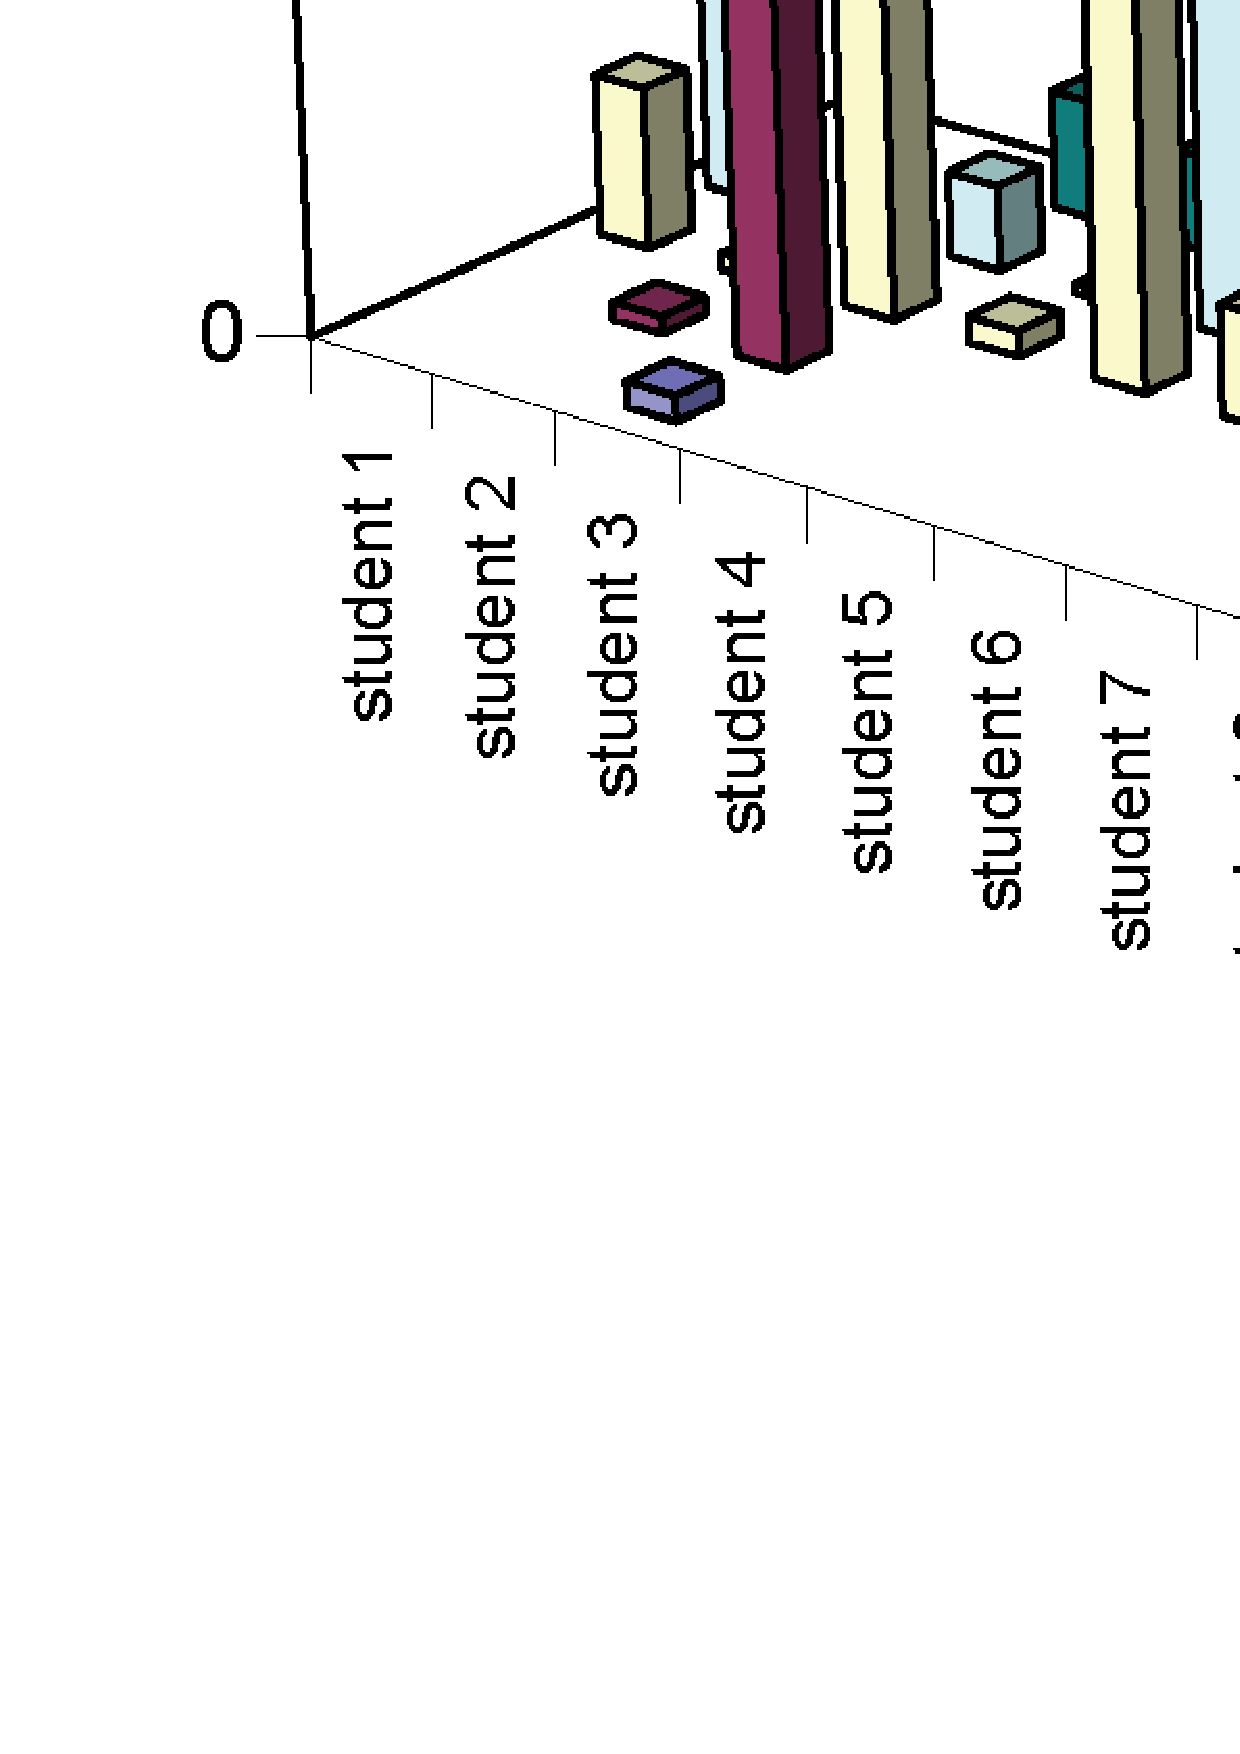
\includegraphics[width=1.00\textwidth]{figures/ClassroomStudyIndividualInvocation}
  \caption{Telemetry Analysis Invocation by Individual and Month} 
  \label{fig:ClassroomStudyIndividualInvocation}
\end{figure}



%%%%%%%%%%%%%%%%%%%%%%%%%%%%%%%%%%%%%%%%%%%%%%%%%%%%%%%%%
%                                                       %
%                   S E C T I O N                       %
%                                                       %
%%%%%%%%%%%%%%%%%%%%%%%%%%%%%%%%%%%%%%%%%%%%%%%%%%%%%%%%%
\clearpage
\section{Study Conclusion}  \label{EvaluationInClassroom:Conclusion}

This study yielded a number of valuable insights into software project telemetry and its implementation.

An automated and unobtrusive metrics collection mechanism is crucial to the success of a metrics program. From the student's feedback, the sensor-based approach appeared to have achieved the goal of eliminating long-term chronic overhead related to metrics collection. However, the one-time setup cost of the sensors was still too high. Though it was not a major issue in the classroom setting, it could cause significant adoption barrier in other environments. Many students had expressed the wish to have an all-in-one intelligent graphical user interface to install and configure the sensors easily. Fortunately, such an installer is now available as a result of user feedback.
	
Software project telemetry appeared to have achieved its design goal of making development process transparent. Most students agreed that they were made more aware of both their own and their team's development process as a result of using the system. However, there was no conclusive evidence to determine whether the increased awareness had actually helped the students improve their software development processes. The data appears to indicate that the ability to understand and interpret telemetry data is related to whether software project telemetry is useful. There were several incidents in which the sensors did not seem to collect metrics correctly, or the telemetry analyses did not seem to compute the data as expected. Some of these were caused by inappropriate interpretation of the results. It seemed that effort-related metrics were most susceptible to mis-interpretation. As far as the implementation was concerned, many students suggested that the web interface for telemetry analysis worked but could be made more user-friendly. 		
	
There was a data privacy issue. Some students seemed to suggest that software project made their development process more transparent than they had wished. They concerned that their personal process data might be misused. I was very well aware of the issue when implementing the system, and had taken steps to limit the kinds of data that could be accessed by people other than the person owning the data. However, it seemed hard to reconcile the conflicting requirements between project management and privacy protection. Some students expressed that they would not want to share personal metrics with others, while other students said they would like to know what other people were doing.

%As with all successful metrics programs, correct interpretation and proper use of metric data are crucial, as well as developer understanding, trust, and support.
	
